\documentclass{article}
\usepackage[utf8]{inputenc}
\usepackage[T1]{fontenc}
\usepackage{amsmath}
\usepackage{graphicx}
\usepackage{physics}
\usepackage{hyperref}
\usepackage{listings}
\usepackage{xcolor}

\title{Importance de l'inclusion des valeurs radiales dans la prédiction du gap par réseau de neurones}
\author{Oussama GUELFAA}
\date{\today}

\begin{document}

\maketitle


\section{Problématique}
Le réseau de neurones actuel utilise uniquement les valeurs d'intensité $I(r)$ comme entrée, sans information explicite sur la position radiale $r$ correspondante. Cette approche présente des limitations fondamentales que nous allons analyser.

\section{Analyse physique du problème}

\subsection{Relation entre gap et fréquence spatiale}
La théorie de Mie qui décrit la formation des anneaux d'intensité établit une relation directe entre le gap et la fréquence spatiale des oscillations. L'intensité normalisée peut s'exprimer comme:

\begin{equation}
\frac{I(r)}{I_{\text{inc}}(r)} = \left| 1 + \frac{E_{\text{scattered}}}{E_{\text{incident}}} \right|^2
\end{equation}

où le terme $\frac{E_{\text{scattered}}}{E_{\text{incident}}}$ dépend explicitement du gap et de la position radiale $r$.

\subsection{Signature du gap dans le profil d'intensité}
La figure \ref{fig:intensity_profile} montre un profil d'intensité typique pour un gap de 0.025 µm et $L_{\text{écran}} = 6.67$ µm.

\begin{figure}[h]
\centering
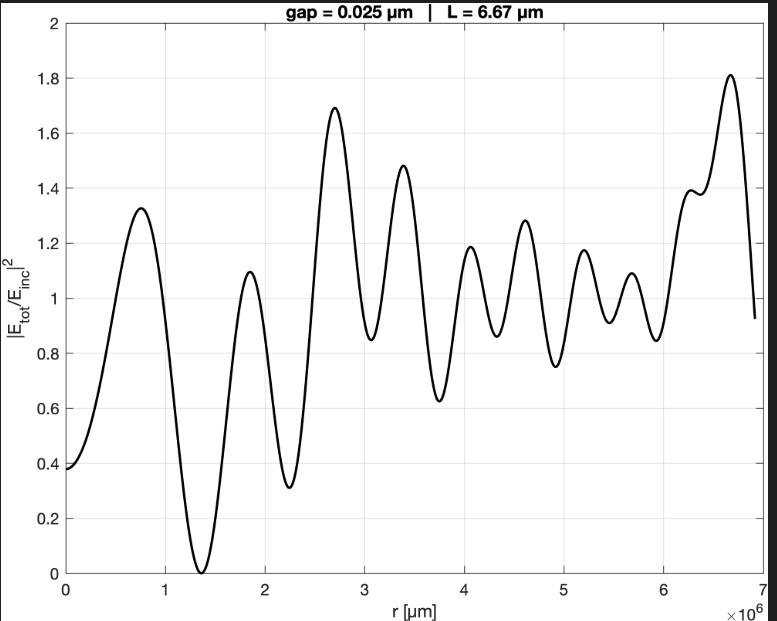
\includegraphics[width=0.8\textwidth]{intensity_profile.png}
\caption{Profil d'intensité radiale pour gap = 0.025 µm et L = 6.67 µm}
\label{fig:intensity_profile}
\end{figure}

On observe que:
\begin{itemize}
    \item La périodicité des oscillations varie avec $r$
    \item L'espacement entre les pics n'est pas constant
    \item L'amplitude des oscillations évolue avec la distance radiale
\end{itemize}

Ces caractéristiques sont des signatures directes du gap et ne peuvent être correctement interprétées sans l'information sur $r$.

\section{Limitations de l'approche actuelle}

\subsection{Problème d'invariance d'échelle}
Sans les valeurs de $r$, le réseau ne peut pas distinguer entre:
\begin{itemize}
    \item Un profil avec oscillations rapprochées sur une grande distance radiale
    \item Un profil avec oscillations éloignées sur une petite distance radiale
\end{itemize}

Ces deux situations correspondent pourtant à des valeurs de gap différentes.

\subsection{Perte d'information physique}
La relation entre la fréquence spatiale des oscillations et le gap est une information physique fondamentale. Sans référence à $r$, cette relation devient inaccessible au réseau.


\section{Solution proposée}

\subsection{Échantillonnage uniforme}
Nous proposons d'utiliser un échantillonnage uniforme de $r$ et d'interpoler les intensités sur cette grille:

\begin{lstlisting}[language=Python, basicstyle=\small\ttfamily, backgroundcolor=\color{gray!10}]
# Créer une grille uniforme
r_uniform = np.linspace(r_min, r_max, 600)

# Interpoler les intensités
I_uniform = np.interp(r_uniform, r_original, I_original)

# Utiliser I_uniform comme entrée du réseau
\end{lstlisting}

Cette approche permet au réseau de comprendre implicitement la relation entre position et intensité, car chaque position dans le vecteur correspond à une valeur $r$ spécifique et connue.

\subsection{Avantages de cette approche}
\begin{itemize}
    \item Préservation de l'information spatiale
    \item Comparabilité entre différents profils
    \item Pas de modification nécessaire de l'architecture du réseau
    \item Cohérence avec la physique du problème
\end{itemize}

\section{Validation théorique}

\subsection{Équation de dispersion}
Pour un système à deux interfaces, la relation de dispersion qui relie le gap $g$ à la fréquence spatiale $k$ des oscillations peut s'approximer par:

\begin{equation}
k \approx \frac{2\pi}{\lambda} \cdot \frac{r}{L} \cdot f(g)
\end{equation}

où $f(g)$ est une fonction du gap. Cette équation montre explicitement que la fréquence spatiale dépend à la fois de $r$ et de $g$.

\subsection{Simulation numérique}
Des simulations numériques confirment que pour deux valeurs de gap différentes, la différence dans les profils d'intensité est principalement visible dans la variation de la fréquence spatiale avec $r$.

\section{Conclusion}
L'inclusion des valeurs de $r$ dans l'entrée du réseau de neurones est essentielle pour la prédiction précise du gap. Cette modification permettra au réseau de capturer la relation physique fondamentale entre la fréquence spatiale des oscillations et le gap, améliorant ainsi significativement les performances du modèle.

\end{document}